% Copyright (C) 2014-2025 by Thomas Auzinger <thomas@auzinger.name>

% Inside the square brackets (e.g., [draft, onside]), different options can be chosen:
% 'draft': Obtain debug information on the build.
% 'final': Remove all debug information in the final build.
% 'onside': Create document for onsided printing (without empty pages added by LaTeX).
% 'twoside': Create document for twosided printing, which adds empty pages to start chapters on odd pages.
\documentclass[twoside]{vutinfth}

% Define convenience functions to use the author name and the thesis title in the PDF document properties.
\newcommand{\authorname}{Artur Ohanian} % The author name without titles.
\newcommand{\thesistitle}{Few-shot Text Line Segmentation for Historical Manuscripts
} % The title of the thesis. The English version should be used, if it exists.

% Create the XMP metadata file for the creation of PDF/A compatible documents.
\begin{filecontents*}[overwrite]{\jobname.xmpdata}
    \Author{\authorname}                                    % The author's name in the document properties.
    \Title{\thesistitle}                                    % The document's title in the document properties.
    \Language{de-AT}                                        % The document's language in the document properties. Select 'en-US', 'en-GB', or 'de-AT'.
    \Keywords{a\sep list\sep of\sep keywords}               % The document's keywords in the document properties (separated by '\sep ').
    \Publisher{TU Wien}                                     % The document's publisher in the document properties.
    \Subject{Thesis}                                        % The document's subject in the document properties.
\end{filecontents*}

% Load packages to allow in- and output of non-ASCII characters.
\usepackage{lmodern}        % Use an extension of the original Computer Modern font to minimize the use of bitmapped letters.
\usepackage[T1]{fontenc}    % Determines font encoding of the output. Font packages have to be included before this line.
\usepackage[utf8]{inputenc} % Determines encoding of the input. All input files have to use UTF8 encoding.

% Extended LaTeX functionality is enabled by including packages with
\usepackage{amsmath}    % Extended typesetting of mathematical expression.
\usepackage{amssymb}    % Provides a multitude of mathematical symbols.
\usepackage{mathtools}  % Further extensions of mathematical typesetting.
\usepackage{microtype}  % Small-scale typographic enhancements.
%\usepackage[inline]{enumitem} % User control over the layout of lists (itemize, enumerate, description).
\usepackage{multirow}   % Allows table elements to span several rows.
\usepackage{float}      % Provides the [H] float placement option.
\usepackage{booktabs}   % Improves the typesetting of tables.
\usepackage{subcaption} % Allows the use of subfigures and enables their referencing.
\usepackage[ruled,linesnumbered,algochapter]{algorithm2e} % Enables the writing of pseudo code.
\usepackage[dvipsnames,table]{xcolor} % Allows the definition and use of colors. This package has to be included before tikz.
\usepackage{nag}        % Issues warnings when best practices in writing LaTeX documents are violated.
\usepackage{todonotes}  % Provides tooltip-like todo notes.
\usepackage{morewrites} % Increases the number of external files that can be used.
\usepackage[a-2b,mathxmp]{pdfx}      % Enables PDF/A compliance. Loads the package hyperref and has to be included second to last.
\usepackage[acronym,toc]{glossaries} % Enables the generation of glossaries and lists of acronyms. This package has to be included last.

% Set PDF document properties
\hypersetup{
    pdfpagelayout   = TwoPageRight,           % How the document is shown in PDF viewers (optional).
    linkbordercolor = {Melon},                % The color of the borders of boxes around hyperlinks (optional).
}

\setpnumwidth{2.5em}        % Avoid overfull hboxes in the table of contents (see memoir manual).
\setsecnumdepth{subsection} % Enumerate subsections.

\nonzeroparskip             % Create space between paragraphs (optional).
\setlength{\parindent}{0pt} % Remove paragraph indentation (optional).

\makeindex      % Use an optional index.
\makeglossaries % Use an optional glossary.
%\glstocfalse   % Remove the glossaries from the table of contents.

% Set persons with 4 arguments:
%  {title before name}{name}{title after name}{gender}
%  where both titles are optional (i.e. can be given as empty brackets {}).
\setauthor{BSc}{\authorname}{Dipl.-Ing.}{male}
\setadvisor{Dipl.-Ing. Dr.techn.}{Florian Kleber}{}{male}

% For bachelor and master theses:
\setfirstassistant{Univ.Ass. BSc MSc ETH}{Rafael Sterzinger}{}{male}
% \setsecondassistant{Pretitle}{Forename Surname}{Posttitle}{male}
% \setthirdassistant{Pretitle}{Forename Surname}{Posttitle}{male}

% For dissertations:
% \setfirstreviewer{Pretitle}{Forename Surname}{Posttitle}{male}
% \setsecondreviewer{Pretitle}{Forename Surname}{Posttitle}{male}

% For dissertations at the PhD School and optionally for dissertations:
% \setsecondadvisor{Pretitle}{Forename Surname}{Posttitle}{male} % Comment to remove.

% Required data.
\setregnumber{12239164}
\setdate{01}{09}{2026} % Set date with 3 arguments: {day}{month}{year}.
\settitle{\thesistitle}{Few-shot Textzeilen Segmentierung für historische Dokumente
} % Sets English and German version of the title (both can be English or German). If your title contains commas, enclose it with additional curvy brackets (i.e., {{your title}}) or define it as a macro as done with \thesistitle
% \setsubtitle{Optional Subtitle of the Thesis}{Optionaler Untertitel der Arbeit} % Sets English and German version of the subtitle (both can be English or German).

% Select the thesis type: bachelor / master / doctor.
% Bachelor:
% \setthesis{bachelor}
%
% Master:
\setthesis{master}
\setmasterdegree{dipl.} % dipl. / rer.nat. / rer.soc.oec. / master
%
% Doctor:
%\setthesis{doctor}
%\setdoctordegree{rer.soc.oec.}% rer.nat. / techn. / rer.soc.oec.

% For bachelor and master:
\setcurriculum{Data Science}{Data Science} % Sets the English and German name of the curriculum.

% Optional reviewer data:
\setfirstreviewerdata{Affiliation, Country}
\setsecondreviewerdata{Affiliation, Country}

\usepackage{subcaption}

\begin{document}

\frontmatter % Switches to roman numbering.
% The structure of the thesis has to conform to the guidelines at
%  https://informatics.tuwien.ac.at/study-services

\addtitlepage{naustrian} % German title page.
\addtitlepage{english} % English title page.
\addstatementpage{english}  % Select 'english' for the English statement text.

% \begin{danksagung*}
% \todo{Ihr Text hier}
% \end{danksagung*}

\begin{acknowledgements*}
    \todo{Enter your text here.}
\end{acknowledgements*}

% \begin{kurzfassung}
% \todo{Ihr Text hier.}
% \end{kurzfassung}

\begin{abstract}
    Text line segmentation is a preprocessing step in the document analysis
    pipeline performed before Optical Character Recognition (OCR) or
    Handwritten Text Recognition (HTR), and its quality directly affects
    recognition performance. For handwritten ancient manuscripts, this task is more
    challenging due to the scarcity of annotated data, degraded image quality,
    and high variability of manuscript layouts and styles.

    This thesis evaluates few-shot training of text line segmentation models
    using three approaches: semantic segmentation, a two-stage detection
    pipeline, and instance segmentation. Under the hypothesis that models with
    convolution-based backbones are inferior in quality, measured by text line
    detection metrics, to models with transformer-based backbones, both architectures are compared across varying sizes and pretrained weights,
    with further fine-tuning on a low number of shots, from 1 to 20.

    \todo{Add paragraph with results description}
\end{abstract}

% Select the language of the thesis, e.g., english or naustrian.
\selectlanguage{english}

% Add a table of contents (toc).
\tableofcontents % Starred version, i.e., \tableofcontents*, removes the self-entry.

% Switch to Arabic numbering and start the enumeration of chapters in the table of contents.
\mainmatter

\chapter{Introduction}

\section{Motivation}
\label{sec:motivation}

\Gls{tls} is an important step in document analysis, since its quality affects downstream text recognition results \cite{fizaine}. For historical manuscripts, this task is particularly challenging for two reasons: physical degradations, such as ink bleeding and faded sections \cite{Rabaev_Litvak_2025}, and varying writing styles both within and between documents, text orientation, and overlapping lines and characters \cite{diva_hisdb}.

Many manuscripts are digitized as images and available online but are not machine-readable; therefore, word searches or text analysis are not possible. Manual labeling is costly and requires expert knowledge and significant time. For example, Tarride et al. \cite{tarride2023handwrittentextrecognitioncrowdsourced} reported that, on average, a crowdsourced annotator took 21 minutes to annotate a full page. Considering the limited availability of labeled data, the \gls{fsl} paradigm can be employed.

\Gls{fsl} is a machine learning paradigm that aims to train models using only a small number of labeled examples per class \cite{fsl}. Unlike traditional supervised learning, which requires fully annotated datasets, \gls{fsl} is designed to generalize from just a few instances, like 1, 3, 5, or 10. It typically relies on two main strategies: meta-learning, which teaches a model how to learn and quickly adapt to new tasks \cite{finn2017modelagnosticmetalearningfastadaptation}, and transfer learning, where a model pre-trained on a large source dataset is fine-tuned for a specific task using limited labeled data \cite{trans_learning}.

In historical document analysis, large source datasets typically contain about 1,500--3,000 annotated document images, such as \gls{cbad} with 3,021 annotated pages \cite{DiemKleberGatos2019} and CATMuS Medieval with 1,705 annotated images \cite{catmus-medieval}. In comparison, ImageNet contains more than 14 million annotated images across over 20,000 object categories \cite{deng2009imagenet}.

For text line segmentation, \gls{fsl} models with transfer learning can rely on pretrained convolutional encoders, such as ResNet, which have been shown to outperform older backbones like VGG-16 in text line segmentation, as shown by the ResNet-50-based Faster R-CNN \cite{jindal2023fasterrcnn}.
\Glspl{vit}, as a next step in computer vision, were reported to outperform them on large-scale recognition benchmarks \cite{dosovitskiy2021imageworth16x16words}, even without using a large amount of data for training \cite{touvron2021trainingdataefficientimagetransformers}. A little later, convolutional networks trained using modern methods reported comparable performance  \cite{liu2022convnet2020s}. More recently, vision foundation models have changed the paradigm: pretrained self-supervised on datasets larger than any annotated collection, they report dense features that surpass supervised
pretraining, and are released with both convolutional and transformer encoders
derived from the same pretraining procedure \cite{oquab2024dinov2learningrobustvisual, darcet2024visiontransformersneedregisters, dinov3, ranzinger2024amradioagglomerativevisionfoundation}. These developments raise the question of the most effective backbone for transfer learning in few-shot models for historical manuscripts, or whether performance depends more on pretraining and on domain-specific or hybrid pretrained backbones, as reported in the adjacent task of document layout analysis \cite{denardin2025indomain}.

\section{Problem Statement}

Although pretrained encoders are widely used for text line segmentation, it remains unclear which encoder architectures best suit few-shot text line segmentation of historical manuscripts. Modern convolutional networks, vision transformers, and vision foundation models differ not only in architecture but also in model size and pretraining data. Therefore, performance differences reported on general computer vision benchmarks may not apply to historical document analysis, especially in few-shot learning settings, which are sensitive to the amount and characteristics of available training data. Robustness across different manuscripts, writing styles, and document conditions is also important to evaluate. These conditions require further investigation.

\section{Objectives}

The main objective of this thesis is to investigate the influence of the encoder on the performance of few-shot text line segmentation models for historical manuscripts. In particular, the thesis aims to:

\begin{itemize}
    \item compare convolution-based and transformer-based encoders across different text line segmentation architectures;
    \item evaluate encoders of different sizes and with different pretraining strategies, including supervised and self-supervised pretraining;
    \item analyze the influence of the number of annotated training images on segmentation performance;
    \item evaluate the robustness of few-shot models across different manuscripts with writing styles and document conditions.
\end{itemize}

\section{Contributions}

The main contributions of this thesis are:

\begin{itemize}
    \item a systematic comparison of modern convolutional and Transformer-based encoders for few-shot text line segmentation of historical manuscripts across different downstream approaches and evaluation settings;
    \item a state-of-the-art-level few-shot text line segmentation model evaluated on a historical manuscript dataset;
    \item a lightweight model pretrained on manuscript data for efficient deployment;
    \item a robustly pretrained model designed to generalize across different manuscripts.
\end{itemize}

\section{Thesis Structure}

The work is organized as follows:

\begin{itemize}
    \item Chapter 2 provides the theoretical background on text line segmentation, describes few-shot learning and its methods, and reviews recent supervised and unsupervised approaches, identifying gaps for research questions.
    \item Chapter 3 formulates research questions.
    \item Chapter 4 describes the methodology for solving the research questions, \gls{fsl} model architectures and parameters (such as backbone weights, postprocessing algorithms, where applicable), experimental design, and text line detection metrics.
    \item Chapter 5 contains quantitative and qualitative results for experiments described in Chapter 4, comparing backbones across tasks of semantic segmentation, object detection, and instance segmentation across various encoder sizes and pretraining options.
    \item Chapter 6 interprets the results, draws conclusions, and answers the research questions.
    \item Chapter 7 summarizes findings and proposes new ideas for extending the few-shot learning paradigm for text line segmentation in historical manuscripts.
\end{itemize}

\chapter{Theoretical Background and Related Work}
\label{lit_rec}

This chapter reviews the domain of historical document analysis and the role of text line segmentation within it,
expands on the theses mentioned in Section \ref{sec:motivation}, describes Few-shot learning essentials, explains how it intersects with text line segmentation in historical documents, and formulates the research gap.

\section{Historical Document Analysis}

Historical document analysis is a research field focused on digitizing, processing, and extracting information from historical documents, whether for content extraction or metadata analysis, such as authorship identification.

\begin{figure}[H]
    \centering
    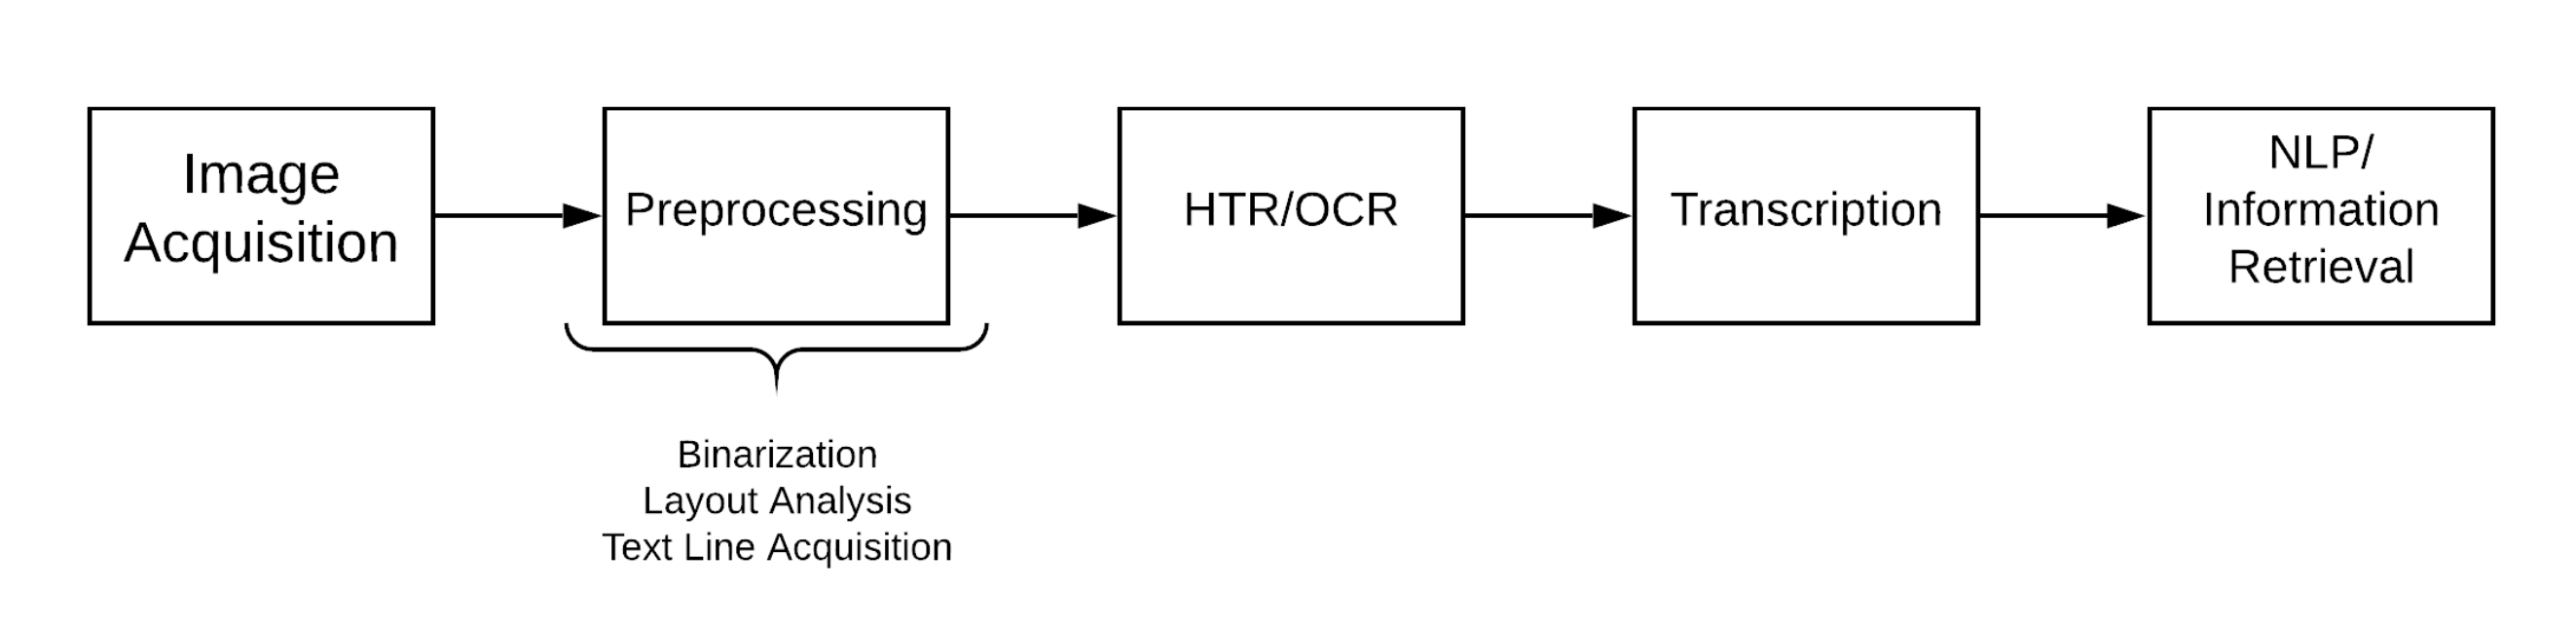
\includegraphics[width=1\linewidth]{graphics/Screenshot from 2026-06-21 13-06-12.png}
    \caption{The steps in a conventional Historical Document Processing workflow for both handwritten and printed documents, reproduced from \cite{DBLP:journals/corr/abs-2002-06300}}
    \label{fig:da_steps}
\end{figure}

Historical document analysis typically involves multiple stages, as shown in Figure \ref{fig:da_steps}. In the pipeline, historical materials pose several challenges because their visual appearance and layout can differ markedly between collections. Frequent issues include uneven line spacing, different text orientations, notes in the margins, stains, bleed-through, and characters or text lines that touch or overlap \cite{Rabaev_Litvak_2025}. Figure \ref{fig:hda_challenges} shows general layout- and degradation-related problems, along with examples of overlapping and deteriorated text line regions.
\begin{figure}[H]
    \centering

    \begin{subfigure}[t]{0.48\linewidth}
        \centering
        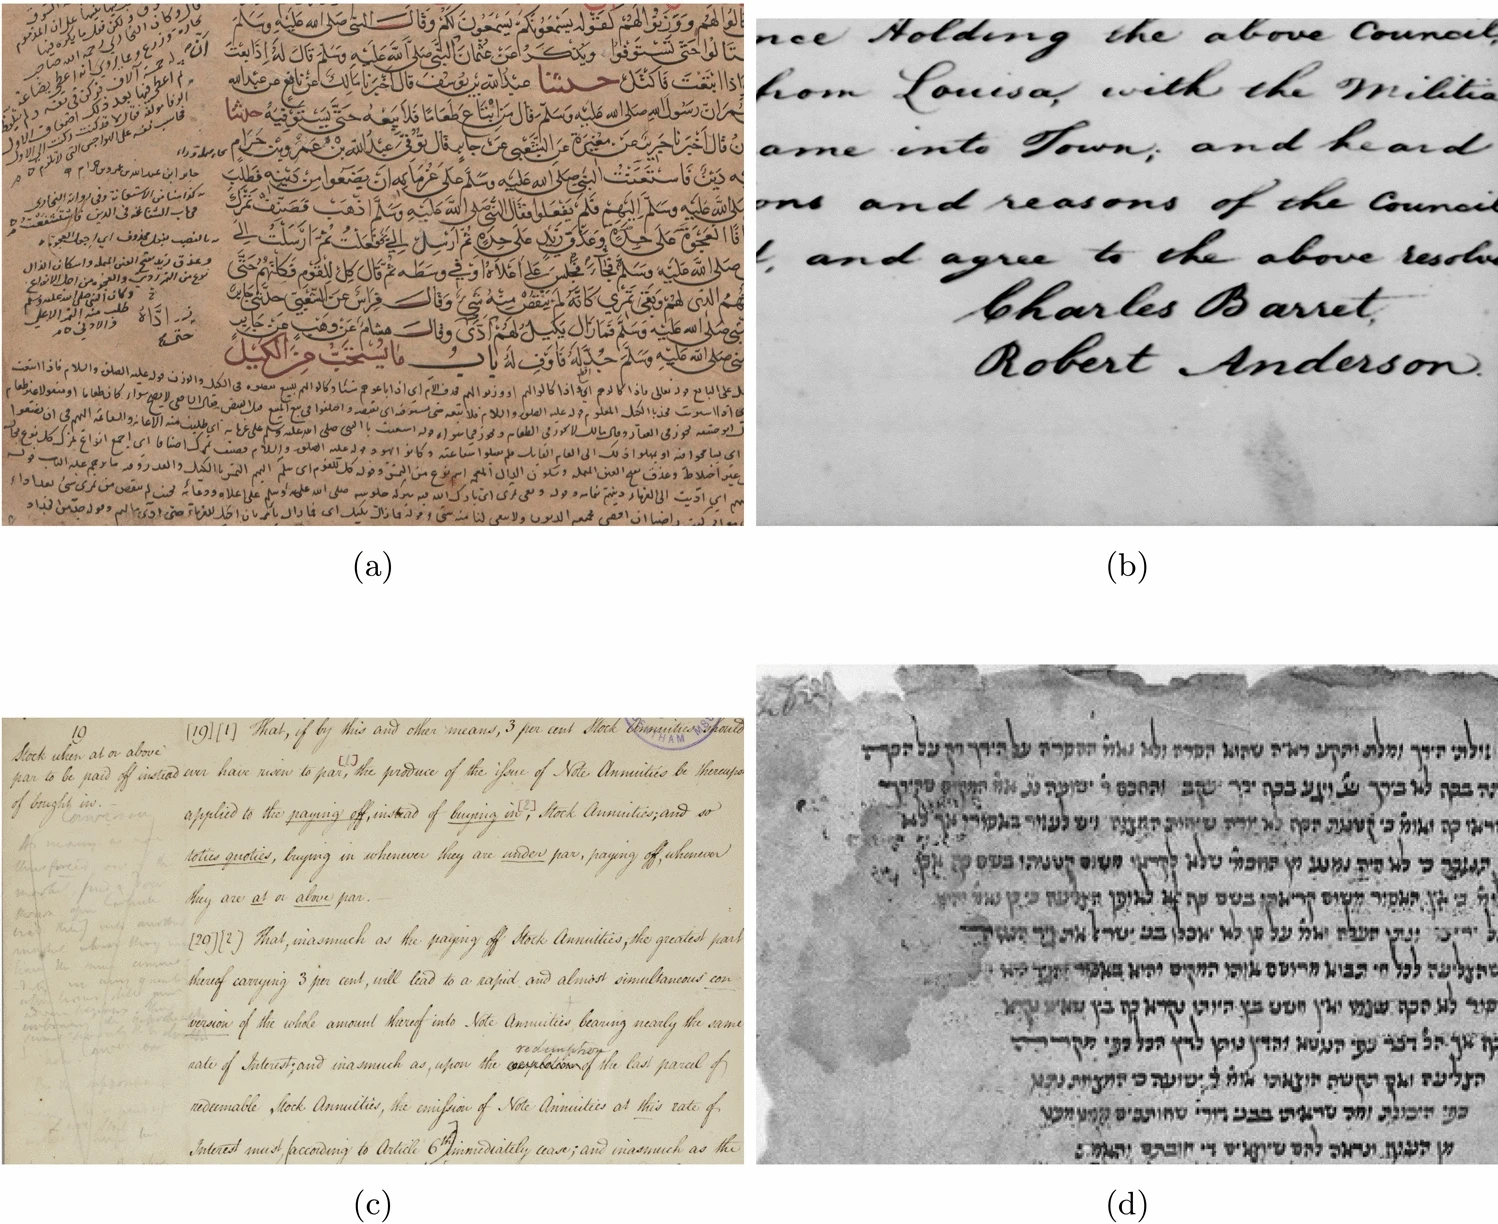
\includegraphics[width=\linewidth]{graphics/deg.png}
        \caption{Challenges in historical document layout analysis: irregular spaces, multi-oriented and fluctuating lines (a); marginal notes (a, c); stains (b, d); touching and connected characters (a, d); bleed-through (c), reproduced from \cite{Rabaev_Litvak_2025}.}
        \label{fig:hda_general_challenges}
    \end{subfigure}
    \hfill
    \begin{subfigure}[t]{0.48\linewidth}
        \centering
        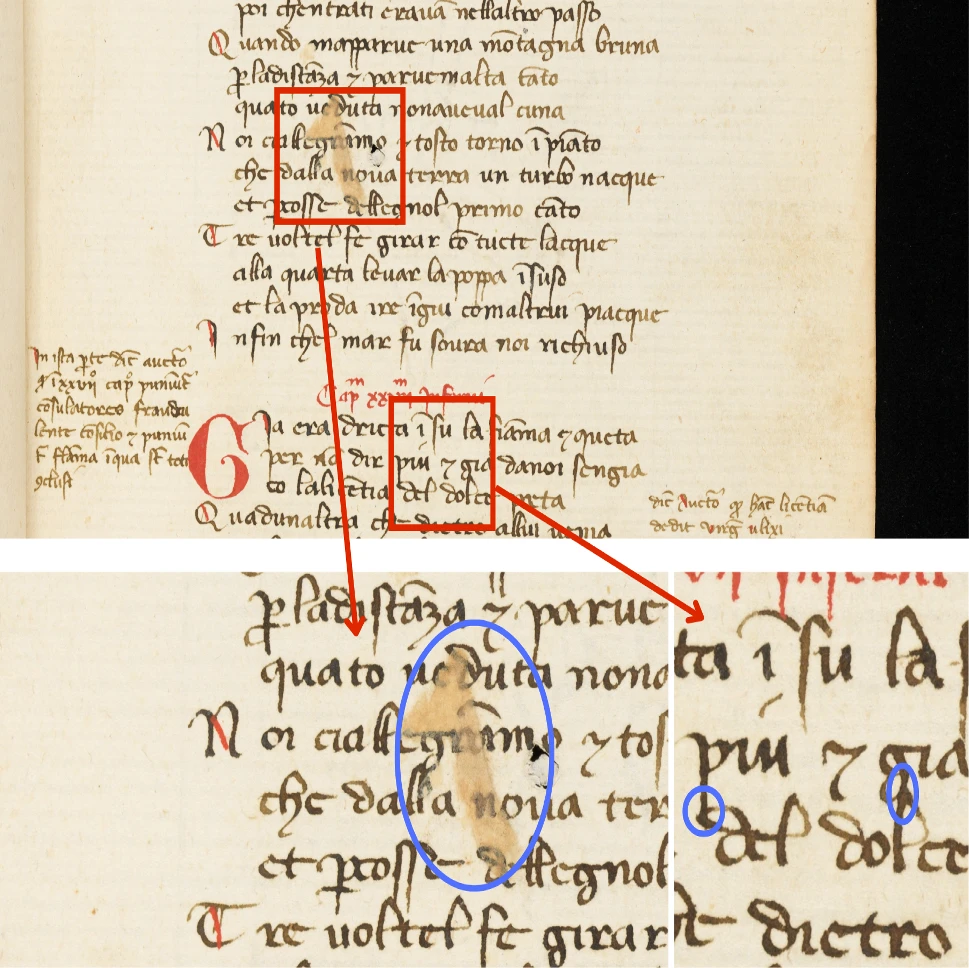
\includegraphics[width=\linewidth]{graphics/cb55_deg.png}
        \caption{Examples of overlapping and degraded text line regions from DIVA-HisDB \cite{diva_hisdb} CB55 subset, reproduced from \cite{Beghoura2026-dp}.}
        \label{fig:hda_line_challenges}
    \end{subfigure}

    \caption{Examples of challenges in text line segmentation in historical documents.}
    \label{fig:hda_challenges}
\end{figure}

Machine learning methods are used at every stage of the processing pipeline. In binarization, machine learning methods generally outperform traditional techniques, even under image degradation and acquisition issues such as uneven lighting; however, they have limitations, including reliance on large, diverse datasets, computational cost, and poor generalization to entirely new document degradations and styles \cite{jimaging11050133}. For document layout analysis, single-branch fully convolutional networks remain the main approach \cite{wu2025hooknet}. However, their reliance on pixel-wise labeled data remains a major limitation, since producing precise ground-truth annotations for historical manuscripts is time-consuming and costly \cite{De_Nardin_2023}. In \gls{htr}, current state-of-the-art approaches are largely transformer-based and tend to perform better on scripts whose handwriting style is similar to what the model was trained on. For instance, Titan and TrOCR-f often perform better out of the box on Latin-script materials, even though script-specific systems trained or fine-tuned on non-Latin data can ultimately achieve higher performance \cite{romein2025htr}. In this task, too, limited labeled domain data remains a key challenge \cite{Li2025}.

As shown in Figure \ref{fig:da_steps}, text line segmentation is the last step in the preprocessing phase; the quality of segmentation affects the performance of the downstream \gls{htr} task. Fizaine et al. measured this effect by comparing two segmentation models with postprocessing, using the same TrOCR \cite{DBLP:journals/corr/abs-2109-10282} detector fine-tuned on the DRoSb dataset, which they also used to train the segmentation models. As shown in Table \ref{tab:fizaine_ap_htr}, the Mask R-CNN \cite{he2017maskrcnn} model has better object-level metrics and also outperforms on the text recognition task, with a lower \gls{cer}.

\begin{table}[h]
    \centering
    \caption{Object-level text line segmentation performance, measured by \gls{ap}, and downstream \gls{htr} performance reported by Fizaine et al. \cite{fizaine}.}
    \label{tab:fizaine_ap_htr}
    \begin{tabular}{lcccc}
        \hline
        Model & \glsentryshort{ap}@0.5 & \glsentryshort{ap}@0.75 & \glsentryshort{ap}@[0.5,0.95] & \glsentryshort{cer} (\%) \\
        \hline
        Doc-UFCN \cite{boillet2021docufcn}
        & 0.62 & 0.52 & 0.50 & 15.3 \\
        Mask R-CNN \cite{he2017maskrcnn}
        & 0.96 & 0.85 & 0.78 & 4.2 \\
        \hline
    \end{tabular}
\end{table}

Text line segmentation is the main focus of this thesis and is discussed in Section~\ref{sec:tls}.

\section{Text Line Segmentation}
\label{sec:tls}

Text line segmentation aims to identify and separate individual text lines in a historical document image. Depending on the labeling method, a text line can be represented as a bounding box, a set of foreground pixels, a polygon surrounding the line, or a baseline. Figure \ref{fig:line_representation} illustrates how different representations describe the same handwritten text lines \cite{Textline_maskrcnn}.

\begin{figure}[H]
    \centering
    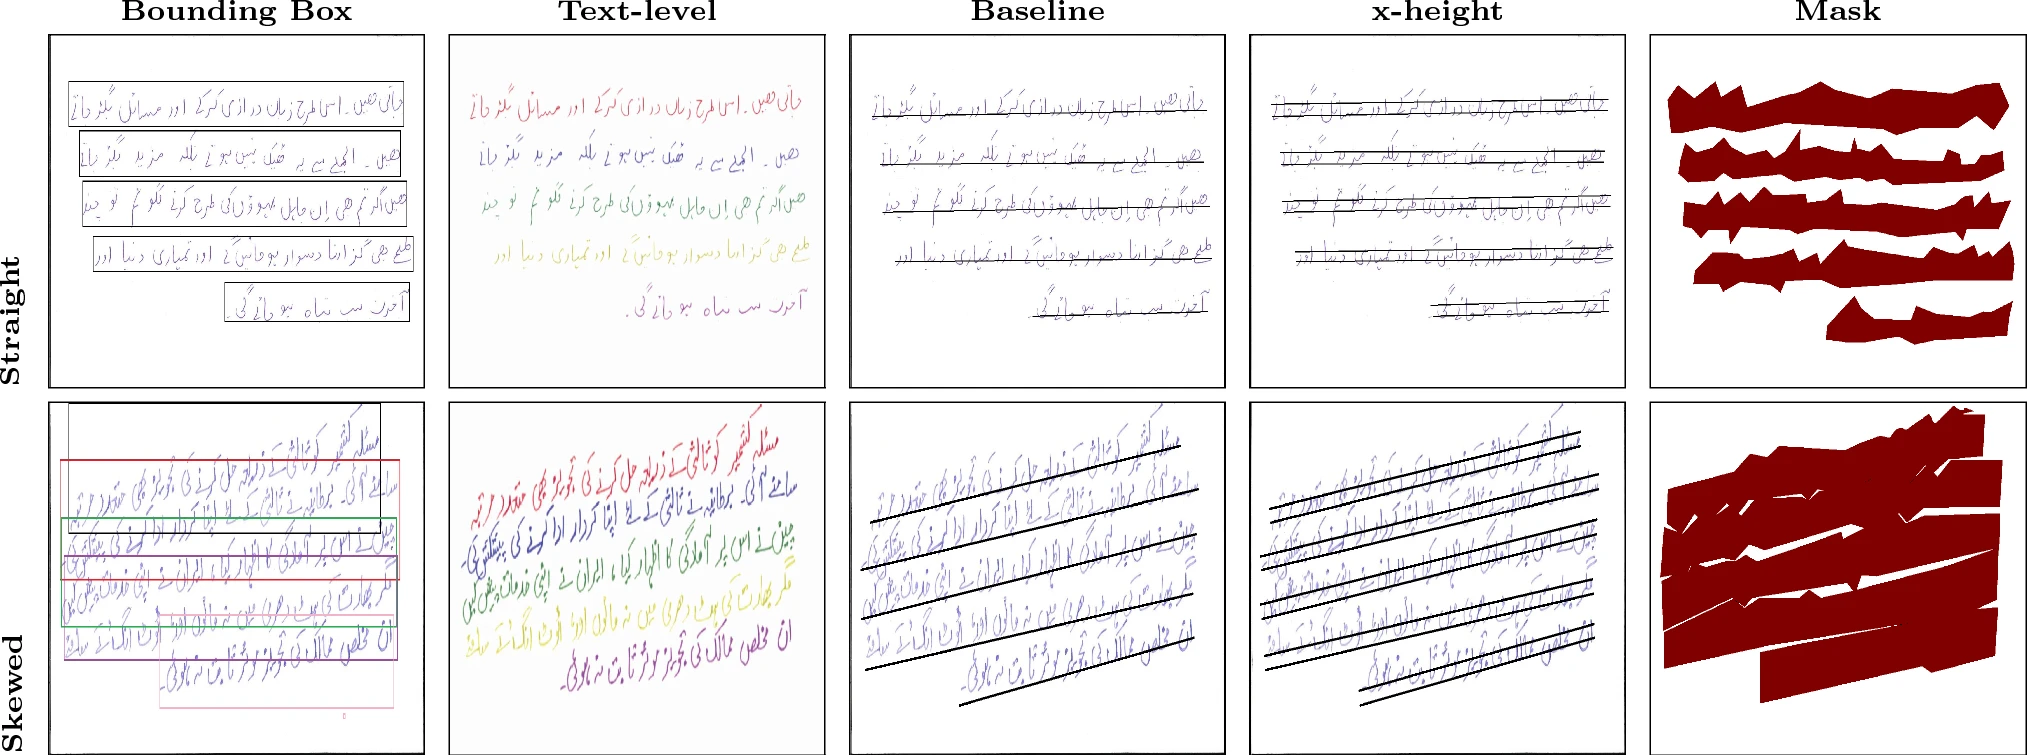
\includegraphics[width=0.85\linewidth]{graphics/tls_r.png}
    \caption{Different representations of a handwritten text line, reproduced from Islam et al. \cite{Textline_maskrcnn}.}
    \label{fig:line_representation}
\end{figure}

\paragraph{Unsupervised Methods} extract individual lines without manually annotated training data, which is very helpful when labeled data for historical documents is limited. The most recent works rely on handcrafted heuristics applied to document structure, such as including elongation analysis for line slicing \cite{sathik2021}, seam carving with specifically designed cost functions \cite{nguyen2022effective}, statistical gap analysis with unsupervised parameter estimation \cite{mukherjee2022unsupervised}, and clustering-based blob-line generation combined with energy minimization \cite{droby2022unsupervised}. Although supervised models are the minority of released models in recent years, as Rabaev et al. \cite{Rabaev_Litvak_2025} report, unsupervised methods achieve performance comparable to and even greater than state-of-the-art models, as can be seen from Table \ref{tab:unsupervised_diva_metrics}. However, their strong performance sometimes depends on the specific assumptions and characteristics of the document collections they are developed for, thus raising the question of whether such methods are robust. Hu et al. \cite{hu2021uchen} propose a method targeted specifically at Uchen Tibetan documents. In contrast, Nguyen et al. \cite{nguyen2022effective} and Droby et al. \cite{droby2022unsupervised} report strong, consistent results across different manuscript families. Additionally, these methods are usually computationally heavy, taking from 4 \cite{droby2022unsupervised} to approximately 30 minutes per page, depending on parameter configuration \cite{DBLP:journals/corr/abs-2003-08632}.

\begin{table}[H]
    \centering
    \caption{Comparison of unsupervised and supervised text line segmentation methods on the DIVA-HisDB \cite{diva_hisdb} dataset using \gls{pixeliu} and \gls{lineiu}.}
    \label{tab:unsupervised_diva_metrics}
    \begin{tabular}{llcc}
        \hline
        Model & Method & \glsentryshort{pixeliu} & \glsentryshort{lineiu} \\
        \hline
        Barakat et al. \cite{DBLP:journals/corr/abs-2003-08632}
        & Unsupervised & 97.50 & \textbf{99.46} \\

        Nguyen et al. \cite{nguyen2022effective}
        & Unsupervised & \textbf{99.36} & 98.86 \\

        Mask R-CNN \cite{Textline_maskrcnn}
        & Supervised & 96.00 & 98.40 \\
        \hline
    \end{tabular}
\end{table}

\paragraph{Supervised Methods} learn text line representations directly from annotated data, allowing them to capture visual characteristics that don't require creating any heuristics. In a recent survey \cite{Rabaev_Litvak_2025},
supervised and hybrid approaches dominate text line segmentation, with more instance segmentation methods published in recent years.

\begin{figure}[H]
    \centering
    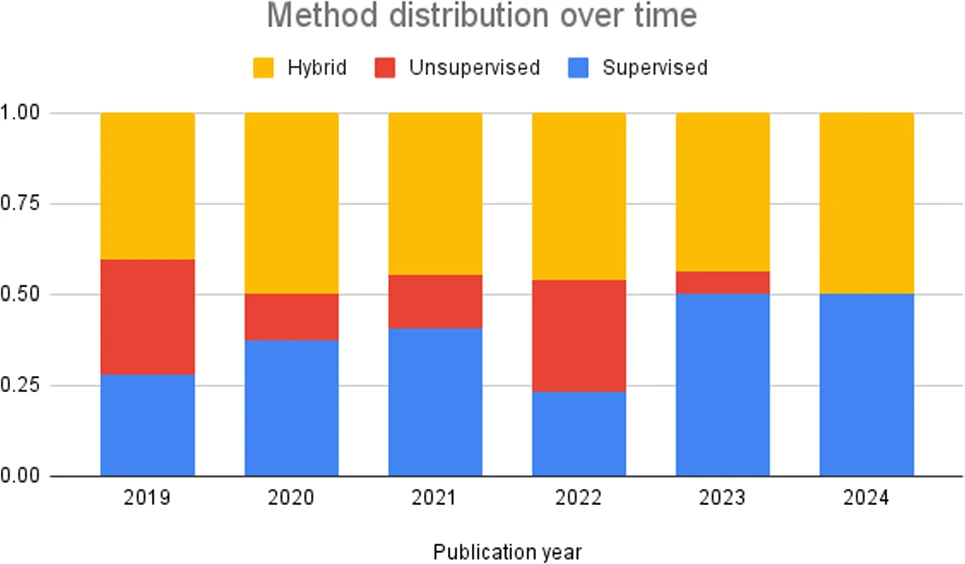
\includegraphics[width=0.85\linewidth]{graphics/sup_m.png}
    \caption{\Gls{tls} for historical manuscripts by approach over time, reproduced from Rabaev et al. \cite{Rabaev_Litvak_2025}.}
    \label{fig:methods}
\end{figure}

Supervised text line segmentation models fall into two categories: semantic segmentation, which may include postprocessing, and instance segmentation. Conventional \gls{fcn}-based models, such as Doc-UFCN \cite{boillet2021docufcn}, formulate the task as a two-class pixelwise classification with classes standing for background and text line. This approach works well when text lines are clearly separated, but neighboring or overlapping lines may be merged into the same foreground region and therefore require additional post-processing. More recent hybrid approaches, such as APAU-Net \cite{Beghoura2026-dp}, keep the semantic segmentation formulation but introduce explicit geometric prior heuristics describing the expected shape, position, and orientation of text lines. Instance segmentation methods address the separation problem differently. For example, Fizaine et al. \cite{fizaine} use Mask R-CNN and treat each text line as a separate object, predicting an individual mask for each detected line; this keeps neighboring lines as separate instances even when their regions are close or partially overlap, and it outperformed convolutional segmentation models, as can be seen from Table \ref{tab:fizaine_instance_comparison}.
\begin{table}[H]
    \centering
    \caption{Object-level text line segmentation performance reported by Fizaine et al. \cite{fizaine}.}
    \label{tab:fizaine_instance_comparison}
    \begin{tabular}{lccc}
        \hline
        Model & \glsentryshort{ap}@0.5 & \glsentryshort{ap}@0.75 & \glsentryshort{ap}@[0.5,0.95] \\
        \hline
        Doc-UFCN \cite{boillet2021docufcn}
        & 0.62 & 0.52 & 0.50 \\

        Mask R-CNN \cite{he2017maskrcnn}
        & \textbf{0.96} & \textbf{0.85} & \textbf{0.78} \\
        \hline
    \end{tabular}
\end{table}

\subparagraph{Robustness} across different scripts and document collections has been evaluated comparatively rarely. Islam et al. \cite{Textline_maskrcnn} study cross-script generalization by training their Mask R-CNN model only on the Urdu HUP dataset and evaluating it on eight other scripts. The model performs reasonably well on documents with layouts similar to the training data, but its performance drops by roughly 20--30\% on datasets with layouts the authors claim are non-similar. The largest failures occur on Arabic and German documents with very low inter-line spacing, showing that differences in page structure can still considerably affect cross-script generalization.

\subparagraph{Learning on a Small Amount of Data} has only recently become a research direction. Zottin et al. \cite{zottin2025exploring} first evaluated three established semantic segmentation architectures---\gls{fcn} \cite{long2015fully}, \gls{pspnet} \cite{zhao2017pyramid}, and DeepLabV3+ \cite{chen2018encoder}---on the U-DIADS-TL dataset, with only 3 annotated images. Their poor results showed rather potential for this field, as it was only baseline research in this paradigm.

The FEST competition \cite{Zottin_2025_FEST} has a wide range of solutions and showed that task-specific approaches can outperform the standard baselines. The winning PERO system used a ParseNet-based line detection pipeline followed by morphological post-processing. Another interesting submission, VAI-OCR, explicitly separated detection and segmentation into two stages: candidate text-line regions were first detected using a DBNet-style approach, after which individual cropped lines were segmented using an ensemble of U-Net and SegFormer models, which is particularly interesting, as to why such an intuitive approach is not used in text line segmentation. This thesis also developed a similar two-stage approach, described in Section \ref{sec:meth}.

U-Net-based architectures demonstrate strong results with very limited training data. Sterzinger et al. \cite{sterzinger2025fewshot} train a lightweight UNet++ model with a connection-aware loss with a \gls{lineiu} of 0.774 on U-DIADS-TL. More recently, APAU-Net \cite{Beghoura2026-dp} combines a residual U-Net with geometric priors and reaches an average \gls{lineiu} of 0.943 under the same three-page training setting.

However, these recent few-shot text line segmentation studies have been developed and evaluated only for the U-DIADS-TL dataset and have not been evaluated on other datasets. This leaves the behavior of few-shot \gls{tls} methods across different historical document collections comparatively underexplored.

\section{Few-shot Learning}
\label{sec:fsl}

\Gls{fsl} aims to learn from a small amount of labeled data \cite{fsl}, where the number of training instances, called shots  \(k\), typically \(k \in \{1,3,5,10\}\). In historical document analysis, this paradigm is highly relevant because of data limitations and the costs of labeling new ones. De Nardin et al. \cite{De_Nardin_2023}, proposed a few-shot framework in adjacent task of historical document layout analysis using only six annotated pages, two from each manuscript, instead of the complete 60-page training set of DIVA-HisDB \cite{diva_hisdb}. The data-poor method achieved performance comparable to data-rich approaches. Additionally, for scene text segmentation in natural images, Li et al. \cite{li2025tsalfewshottextsegmentation} proposed a model that creates prior knowledge from the pretrained \gls{clip} model \cite{DBLP:journals/corr/abs-2103-00020} to learn text attributes from only a few labeled images. On the TextSeg dataset \cite{xu2020rethinkingtextsegmentationnovel}, their 4-shot setting outperforms several many-shot baselines trained with up to 128 labeled examples, demonstrating the potential of few-shot methods for data-efficient text segmentation, even though the work is outside the historical document analysis domain. \Gls{fsl} can be applied in two approaches: meta-learning, where a model is trained to adapt rapidly to new tasks from a small support set, and transfer learning, where knowledge learned from a larger source dataset is reused for a target task with limited labeled data \cite{fsl}.

\paragraph{Transfer Learning using Pretrained Backbones}
 In deep neural networks, transfer learning is commonly implemented by initializing the model's feature extractor (i.e., the backbone/encoder) with pretrained weights and then adapting these weights to the target task through a brief training process called fine-tuning \cite{plested2026transfer}. This approach lets the feature extractor adjust representations learned from a larger source dataset rather than learning them entirely from limited target data.
 
Transfer Learning using Pretrained Backbones is available with both \glspl{cnn} and transformer-based models. ResNet-derived \glspl{cnn} have been adopted as generic feature extractors, whereas \Glspl{vit} have demonstrated state-of-the-art performance on large-scale computer vision benchmarks \cite{dosovitskiy2021imageworth16x16words}. Subsequent work on data-efficient training strategies further enhanced \gls{vit} performance under limited-data regimes \cite{touvron2021trainingdataefficientimagetransformers}. In parallel, ConvNeXt established that appropriately modernized convolutional architectures can achieve performance comparable to transformer-based approaches \cite{liu2022convnet2020s,woo2023convnextv2}. Later, self-supervised vision foundation models have provided general-purpose pretrained representations. DINOv2 uses \gls{vit} encoders pretrained on the LVD-142M dataset and provides features suitable for dense prediction tasks \cite{oquab2024dinov2learningrobustvisual,darcet2024visiontransformersneedregisters}. DINOv3 extends this family with both \gls{vit} and ConvNeXt encoders trained using the same self-supervised framework \cite{dinov3}.

Experiments with different backbones have also been performed in historical document analysis. Wödlinger and Sablatnig use an ImageNet-pretrained ResNet-50 as the encoder of a U-Net-based baseline detection system and report an F1 score of 0.881 on cBAD2019 \cite{wodlinger2021baseline}. Their experiments further show that improving the initial phase of model estimation improves final performance, with the F1 score increasing by ~10\% to 0.963 when ground-truth start points and angles are provided. Jindal and Ghosh \cite{jindal2023fasterrcnn} further replaced the conventional VGG-16 backbone of Faster R-CNN with ResNet-50 for ancient handwritten text line segmentation and report an F-measure of 99.98\%, outperforming the original Faster R-CNN configuration. Fizaine et al. \cite{fizaine} also suggest replacing the backbone in their Mask R-CNN implementation with a more recent architecture, such as ConvNeXt \cite{woo2023convnextv2}, to potentially improve both accuracy and processing speed. These works suggest room for extensive research on \gls{tls} backbones.
The source of pretraining also matters. Common backbones are pretrained on large
datasets such as ImageNet \cite{deng2009imagenet} and \gls{coco} \cite{DBLP:journals/corr/LinMBHPRDZ14}, whereas historical document datasets such as \gls{cbad} \cite{cbad-2019} and CATMuS \cite{catmus-medieval} are substantially smaller but closer to the target domain. Table \ref{tab:pretraining_datasets} demonstrates an order-of-magnitude difference between the generic and task-specific datasets.

\begin{table}[H]
    \centering
    \caption{Size comparison of generic computer vision and historical document datasets relevant for pretraining.}
    \label{tab:pretraining_datasets}
    \begin{tabular}{llr}
        \hline
        Dataset & Domain & Number of images/pages \\
        \hline
        ImageNet \cite{deng2009imagenet}
        & Natural images & 14,197,122 images \\

        ImageNet-1K
        & Natural images & 1,281,167 images \\

        \gls{coco} \cite{DBLP:journals/corr/LinMBHPRDZ14}
        & Natural images & 328,000 images \\

        \gls{cbad} 2019 \cite{cbad-2019}
        & Historical documents & 3,021 pages \\

        CATMuS Medieval \cite{catmus-medieval}
        & Historical documents & 1,705 images \\
        \hline
    \end{tabular}
\end{table}

Domain-specific encoder pretraining remains unexplored for \gls{tls}. De Nardin et al. \cite{denardin2025indomain} show that pretraining source strongly affects historical document layout analysis. On CB55, training from scratch yields 43.9\% \gls{iou} and 57.6\% F1; hybrid \gls{coco}+U-DIADS-Bib pretraining raises this to 50.8\% \gls{iou} and 65.1\% F1 with a frozen encoder, and 54.6\% \gls{iou} and 69.0\% F1 after fine-tuning—gains of up to +10.7 \gls{iou} and +11.4 F1 points, proving the potential of this approach for \gls{tls}.

\section{Summary of Studies and Research Gap}

Recent work therefore suggests that both encoder architecture and pretraining strategy can affect performance under limited data. However, a systematic comparison of modern convolutional, Transformer-based, and vision-foundation-model encoders under the same few-shot text line segmentation setting, alongside different encoder pretraining options, remains unexplored, although these methods are used for adjacent tasks in historical layout analysis. This motivates the controlled comparison in this thesis, with the \glspl{rq} stated in Section \ref{ch:rqs}.

\chapter{Research Questions}
\label{ch:rqs}
\glsreset{rq}
Based on the challenges in the field of text line segmentation and after conducting a literature review in Chapter \ref{lit_rec} and considering its conclusions, several \glspl{rq} were formulated:

\begin{enumerate}
    \item How well, in terms of the line detection metrics, does an \gls{fsl} model using a transformer-based backbone perform compared to a \gls{cnn} backbone for text line segmentation in historical manuscripts?
    \item How many labeled images are needed to achieve performance comparable to \gls{sota} methods, as measured by the line detection metrics?
    \item How do the heterogeneity and quality (e.g., Latin-only vs. mixed scripts; clean vs. mixed clean and degraded vs. only degraded) of training documents affect the performance of a text line segmentation model, i.e., does manuscript diversity impact \gls{fsl} model robustness?
\end{enumerate}

The line detection metrics mentioned in \gls{rq}1 and used for evaluation are described in Section \ref{metrics}.

\chapter{Methodology}
\label{sec:meth}
\section{Datasets}

\todo{list all dataset for all 3 RQs, add some additional info}

\section{Evaluation Metrics}
\label{metrics}

\todo{to rewrite metrics}

Evaluation is performed using Input over Output (IU) metrics from Task 3 of ICDAR 2017 Competition on Layout Analysis for Challenging Medieval Manuscripts~\cite{metrics_iu}, computed with the freely available DIVA Line Segmentation Evaluator~\cite{diva_tool}, and other 3 metrics follow the Handwriting Segmentation Contest Protocol ~\cite{metrics_hscp}:

\begin{enumerate}
    \item Pixel Intersection over Union (Pixel IU): evaluates overlap between predicted and ground-truth at the pixel level. It is defined as
    \[ \text{Pixel IU} = \frac{TP}{TP + FP + FN} \]
    where TP are correctly predicted text pixels, FP are extra predicted pixels, and FN are missed text pixels.

    \item Line Intersection over Union (Line IU): evaluates overlap at the line level using the same IoU formula:
    \[ \text{Line IU} = \frac{TP}{TP + FP + FN} \]
    Here, TP is the number of matched lines, FP are spurious lines, and FN are missed lines. A predicted line matches ground truth if both pixel-level precision and recall exceed 75\%.

    \item Detection Rate (DR): proportion of matched ground-truth lines:
    \[ \text{DR} = \frac{M}{N_1} \]
    where \( M \) is the number of one-to-one matched lines, computed based on threshold 75\% and \( N_1 \) is the number of ground-truth lines.

    \item Recognition Accuracy (RA): proportion of matched predicted lines:
    \[ \text{RA} = \frac{M}{N_2} \]
    where \( N_2 \) is the number of predicted lines.

    \item F-Measure (FM): harmonic mean of DR and RA:
    \[ \text{FM} = \frac{2 \cdot \text{DR} \cdot \text{RA}}{\text{DR} + \text{RA}} \]
\end{enumerate}

\todo[inline]{add model desctiptions: simple seg}
\todo[inline]{add model desctiptions: 2stage}
\todo[inline]{add model desctiptions: 2stage detector distillation and pretraining}
\todo[inline]{add model desctiptions: mask2former}
\todo[inline]{add shot sampling strategies}
\todo[inline]{add rq3 cross validation strategies}

\chapter{Experiments \& Results}

\todo[inline]{1. Simple segmentation(U-net, Segformer, backbones, qualitative asessment}
\todo[inline]{2. Two-stage(Yolo vs DETR)}
\todo[inline]{2. Two-stage detector pretraining}
\todo[inline]{3. Mask2former}
\todo[inline]{4. Effect on number of shots(U-Net, two-stage, mask2former}
\todo[inline]{5. Cross validation results)}

\section{RQ1: CNN vs. ViT Backbone Comparison}

\subsection{Semantic Segmentation}

% Latin14396
\begin{table}[H]
    \centering
    \caption{Results on the Latin14396 subset.}
    \label{tab:latin14396}
    \begin{tabular}{llclccccc}
        \hline
        Encoder & Init & Bucket & Params, M &
        Pixel IU & Line IU & DR & RA & FM \\
        \hline
        vit\_tiny        & imagenet & XS & 5.5  & \textbf{0.85} & 0.96 & 0.95 & 0.93 & 0.94 \\
        vit\_tiny        & random   & XS & 5.5  & \textbf{0.85} & 0.97 & 0.95 & 0.91 & 0.93 \\
        convnext\_femto  & imagenet & XS & 4.83 & 0.84 & 0.97 & 0.95 & 0.95 & 0.95 \\
        convnext\_femto  & random   & XS & 4.83 & 0.83 & 0.96 & 0.94 & 0.89 & 0.91 \\
        pvt\_v2\_b0      & imagenet & XS & 3.41 & 0.84 & 0.97 & 0.95 & 0.94 & 0.95 \\
        pvt\_v2\_b0      & random   & XS & 3.41 & 0.83 & 0.96 & 0.94 & 0.89 & 0.91 \\
        convnext\_pico   & imagenet & S  & 8.53 & 0.84 & 0.97 & 0.95 & 0.94 & 0.94 \\
        convnext\_pico   & random   & S  & 8.53 & 0.83 & 0.96 & 0.94 & 0.91 & 0.92 \\
        pvt\_v2\_b1      & imagenet & S  & 13.5 & 0.84 & 0.97 & \textbf{0.96} & 0.95 & \textbf{0.96} \\
        pvt\_v2\_b1      & random   & S  & 13.5 & 0.83 & 0.96 & 0.93 & 0.89 & 0.91 \\
        convnext\_tiny   & dinov3   & M  & 27.8 & 0.83 & 0.96 & 0.94 & 0.93 & 0.93 \\
        convnext\_tiny   & imagenet & M  & 27.8 & \textbf{0.85} & 0.97 & \textbf{0.96} & \textbf{0.96} & \textbf{0.96} \\
        convnext\_tiny   & random   & M  & 27.8 & 0.84 & 0.96 & 0.94 & 0.90 & 0.92 \\
        vit\_small       & dinov3   & M  & 21.7 & \textbf{0.85} & \textbf{0.98} & 0.95 & 0.95 & 0.95 \\
        vit\_small       & imagenet & M  & 21.7 & \textbf{0.85} & 0.96 & 0.95 & 0.94 & 0.94 \\
        vit\_small       & random   & M  & 21.7 & \textbf{0.85} & 0.96 & 0.95 & 0.92 & 0.93 \\
        pvt\_v2\_b2      & imagenet & M  & 24.9 & 0.84 & 0.97 & \textbf{0.96} & 0.95 & 0.95 \\
        pvt\_v2\_b2      & random   & M  & 24.9 & 0.83 & 0.96 & 0.94 & 0.89 & 0.91 \\
        \hline
    \end{tabular}
\end{table}

% Latin2
\begin{table}[h]
    \centering
    \caption{Results on the Latin2 subset.}
    \label{tab:latin2}
    \begin{tabular}{llclccccc}
        \hline
        Encoder & Init & Bucket & Params, M &
        Pixel IU & Line IU & DR & RA & FM \\
        \hline
        vit\_tiny        & imagenet & XS & 5.5  & 0.81 & 0.96 & 0.86 & 0.85 & 0.85 \\
        vit\_tiny        & random   & XS & 5.5  & 0.81 & 0.96 & 0.83 & 0.84 & 0.83 \\
        convnext\_femto  & imagenet & XS & 4.83 & 0.81 & 0.96 & 0.87 & 0.88 & 0.87 \\
        convnext\_femto  & random   & XS & 4.83 & 0.79 & 0.95 & 0.82 & 0.76 & 0.78 \\
        pvt\_v2\_b0      & imagenet & XS & 3.41 & 0.80 & 0.96 & 0.86 & 0.87 & 0.86 \\
        pvt\_v2\_b0      & random   & XS & 3.41 & 0.79 & 0.96 & 0.84 & 0.80 & 0.82 \\
        convnext\_pico   & imagenet & S  & 8.53 & \textbf{0.83} & 0.97 & \textbf{0.89} & \textbf{0.92} & \textbf{0.90} \\
        convnext\_pico   & random   & S  & 8.53 & 0.79 & 0.94 & 0.83 & 0.78 & 0.80 \\
        pvt\_v2\_b1      & imagenet & S  & 13.5 & 0.82 & 0.97 & 0.88 & 0.91 & 0.89 \\
        pvt\_v2\_b1      & random   & S  & 13.5 & 0.80 & 0.94 & 0.83 & 0.77 & 0.80 \\
        convnext\_tiny   & dinov3   & M  & 27.8 & 0.81 & 0.97 & 0.87 & 0.89 & 0.88 \\
        convnext\_tiny   & imagenet & M  & 27.8 & 0.82 & 0.97 & 0.88 & 0.89 & 0.88 \\
        convnext\_tiny   & random   & M  & 27.8 & 0.80 & 0.94 & 0.84 & 0.78 & 0.81 \\
        vit\_small       & dinov3   & M  & 21.7 & \textbf{0.83} & 0.97 & 0.88 & 0.91 & 0.89 \\
        vit\_small       & imagenet & M  & 21.7 & 0.81 & 0.96 & 0.86 & 0.81 & 0.83 \\
        vit\_small       & random   & M  & 21.7 & 0.82 & \textbf{0.98} & 0.86 & 0.85 & 0.85 \\
        pvt\_v2\_b2      & imagenet & M  & 24.9 & 0.81 & 0.97 & 0.87 & 0.89 & 0.88 \\
        pvt\_v2\_b2      & random   & M  & 24.9 & 0.79 & 0.93 & 0.82 & 0.75 & 0.78 \\
        \hline
    \end{tabular}
\end{table}

% Syr341
\begin{table}[H]
    \centering
    \caption{Results on the Syr341 subset.}
    \label{tab:syr341}
    \begin{tabular}{llclccccc}
        \hline
        Encoder & Init & Bucket & Params, M &
        Pixel IU & Line IU & DR & RA & FM \\
        \hline
        vit\_tiny        & imagenet & XS & 5.5  & 0.73 & 0.90 & 0.75 & 0.75 & 0.75 \\
        vit\_tiny        & random   & XS & 5.5  & \textbf{0.74} & 0.90 & 0.72 & 0.71 & 0.71 \\
        convnext\_femto  & imagenet & XS & 4.83 & 0.69 & 0.88 & 0.74 & 0.77 & 0.75 \\
        convnext\_femto  & random   & XS & 4.83 & 0.71 & 0.88 & 0.58 & 0.55 & 0.57 \\
        pvt\_v2\_b0      & imagenet & XS & 3.41 & 0.73 & 0.90 & 0.76 & 0.78 & 0.77 \\
        pvt\_v2\_b0      & random   & XS & 3.41 & 0.71 & 0.88 & 0.68 & 0.66 & 0.67 \\
        convnext\_pico   & imagenet & S  & 8.53 & 0.72 & 0.89 & \textbf{0.77} & 0.78 & 0.77 \\
        convnext\_pico   & random   & S  & 8.53 & 0.72 & 0.88 & 0.69 & 0.67 & 0.67 \\
        pvt\_v2\_b1      & imagenet & S  & 13.5 & 0.71 & 0.89 & \textbf{0.77} & \textbf{0.79} & \textbf{0.78} \\
        pvt\_v2\_b1      & random   & S  & 13.5 & 0.73 & 0.90 & 0.71 & 0.69 & 0.70 \\
        convnext\_tiny   & dinov3   & M  & 27.8 & 0.71 & 0.88 & 0.75 & 0.78 & 0.77 \\
        convnext\_tiny   & imagenet & M  & 27.8 & 0.72 & 0.89 & \textbf{0.77} & \textbf{0.79} & \textbf{0.78} \\
        convnext\_tiny   & random   & M  & 27.8 & 0.72 & 0.89 & 0.68 & 0.66 & 0.67 \\
        vit\_small       & dinov3   & M  & 21.7 & \textbf{0.74} & \textbf{0.92} & 0.74 & 0.75 & 0.75 \\
        vit\_small       & imagenet & M  & 21.7 & 0.73 & 0.90 & 0.74 & 0.75 & 0.75 \\
        vit\_small       & random   & M  & 21.7 & 0.72 & 0.89 & 0.70 & 0.70 & 0.70 \\
        pvt\_v2\_b2      & imagenet & M  & 24.9 & 0.72 & 0.89 & \textbf{0.77} & \textbf{0.79} & \textbf{0.78} \\
        pvt\_v2\_b2      & random   & M  & 24.9 & 0.73 & 0.90 & 0.69 & 0.67 & 0.68 \\
        \hline
    \end{tabular}
\end{table}

% Average over all subsets
\begin{table}[H]
    \centering
    \caption{Average results across Latin14396, Latin2, and Syr341 subsets.}
    \label{tab:udiads_average}
    \begin{tabular}{llclccccc}
        \hline
        Encoder & Init & Bucket & Params, M &
        Pixel IU & Line IU & DR & RA & FM \\
        \hline
        vit\_tiny        & imagenet & XS & 5.5  & 0.80 & 0.94 & 0.85 & 0.84 & 0.85 \\
        vit\_tiny        & random   & XS & 5.5  & 0.80 & 0.94 & 0.83 & 0.82 & 0.82 \\
        convnext\_femto  & imagenet & XS & 4.83 & 0.78 & 0.94 & 0.85 & 0.87 & 0.86 \\
        convnext\_femto  & random   & XS & 4.83 & 0.78 & 0.93 & 0.78 & 0.73 & 0.75 \\
        pvt\_v2\_b0      & imagenet & XS & 3.41 & 0.79 & 0.94 & 0.86 & 0.86 & 0.86 \\
        pvt\_v2\_b0      & random   & XS & 3.41 & 0.78 & 0.93 & 0.82 & 0.78 & 0.80 \\
        convnext\_pico   & imagenet & S  & 8.53 & 0.80 & 0.94 & \textbf{0.87} & \textbf{0.88} & 0.87 \\
        convnext\_pico   & random   & S  & 8.53 & 0.78 & 0.93 & 0.82 & 0.79 & 0.80 \\
        pvt\_v2\_b1      & imagenet & S  & 13.5 & 0.79 & 0.94 & \textbf{0.87} & \textbf{0.88} & \textbf{0.88} \\
        pvt\_v2\_b1      & random   & S  & 13.5 & 0.79 & 0.93 & 0.82 & 0.78 & 0.80 \\
        convnext\_tiny   & dinov3   & M  & 27.8 & 0.78 & 0.94 & 0.85 & 0.87 & 0.86 \\
        convnext\_tiny   & imagenet & M  & 27.8 & 0.80 & 0.94 & \textbf{0.87} & \textbf{0.88} & 0.87 \\
        convnext\_tiny   & random   & M  & 27.8 & 0.79 & 0.93 & 0.82 & 0.78 & 0.80 \\
        vit\_small       & dinov3   & M  & 21.7 & \textbf{0.81} & \textbf{0.96} & 0.86 & 0.87 & 0.86 \\
        vit\_small       & imagenet & M  & 21.7 & 0.80 & 0.94 & 0.85 & 0.83 & 0.84 \\
        vit\_small       & random   & M  & 21.7 & 0.80 & 0.94 & 0.84 & 0.82 & 0.83 \\
        pvt\_v2\_b2      & imagenet & M  & 24.9 & 0.79 & 0.94 & \textbf{0.87} & \textbf{0.88} & 0.87 \\
        pvt\_v2\_b2      & random   & M  & 24.9 & 0.78 & 0.93 & 0.82 & 0.77 & 0.79 \\
        \hline
    \end{tabular}
\end{table}

% Average by parameter bucket
\begin{table}[H]
    \centering
    \caption{Average results by model size across the entire U-DIADS-TL dataset.}
    \label{tab:udiads_bucket_average}
    \begin{tabular}{lcccccc}
        \hline
        Bucket & Params, M & Pixel IU & Line IU & DR & RA & FM \\
        \hline
        XS & 4.58  & \textbf{0.79} & \textbf{0.94 }& 0.83 & 0.82 & 0.82 \\
        S  & 11.02 & \textbf{0.79} & \textbf{0.94} & \textbf{0.85} & 0.83 & \textbf{0.84} \\
        M  & 24.79 & \textbf{0.79} & \textbf{0.94} & \textbf{0.85} & \textbf{0.84} & \textbf{0.84} \\
        \hline
    \end{tabular}
\end{table}

\begin{table}[H]
    \centering
    \caption{Average results by architecture family and initialization across the entire U-DIADS-TL dataset.}
    \label{tab:udiads_family_init_average}
    \begin{tabular}{llcccccc}
        \hline
        Model & Init & Params, M & Pixel IU & Line IU & DR & RA & FM \\
        \hline
        ViT      & dinov3   & 21.70 & \textbf{0.81} & \textbf{0.96} & 0.86 & 0.87 & 0.86 \\
        ViT      & imagenet & 13.60 & 0.80 & 0.94 & 0.85 & 0.84 & 0.84 \\
        ViT      & random   & 13.60 & 0.80 & 0.94 & 0.84 & 0.82 & 0.82 \\
        \hline
        PVT      & imagenet & 13.94 & 0.79 & 0.94 & \textbf{0.87} & 0.87 & \textbf{0.87} \\
        PVT      & random   & 13.94 & 0.78 & 0.93 & 0.82 & 0.78 & 0.80 \\
        \hline
        ConvNeXt & dinov3   & 27.80 & 0.78 & 0.94 & 0.85 & 0.87 & 0.86 \\
        ConvNeXt & imagenet & 13.72 & 0.79 & 0.94 & 0.86 & \textbf{0.88} & \textbf{0.87} \\
        ConvNeXt & random   & 13.72 & 0.78 & 0.93 & 0.81 & 0.77 & 0.78 \\
        \hline
    \end{tabular}
\end{table}

% Average by parameter bucket and initialization
\begin{table}[H]
    \centering
    \caption{Average results by model size and initialization across the entire U-DIADS-TL dataset.}
    \label{tab:udiads_bucket_init_average}
    \begin{tabular}{llcccccc}
        \hline
        Bucket & Init & Params, M & Pixel IU & Line IU & DR & RA & FM \\
        \hline
        XS & imagenet & 4.58  & 0.79 & 0.94 & 0.85 & 0.86 & 0.86 \\
        XS & random   & 4.58  & 0.79 & 0.93 & 0.81 & 0.78 & 0.79 \\
        \hline
        S  & imagenet & 11.02 & 0.80 & 0.94 & \textbf{0.87} & \textbf{0.88} & \textbf{0.88} \\
        S  & random   & 11.02 & 0.79 & 0.93 & 0.82 & 0.79 & 0.80 \\
        \hline
        M  & dinov3   & 24.75 & 0.80 & \textbf{0.95} & 0.86 & 0.87 & 0.86 \\
        M  & imagenet & 24.80 & \textbf{0.80} & 0.94 & 0.86 & 0.86 & 0.86 \\
        M  & random   & 24.80 & 0.79 & 0.93 & 0.83 & 0.79 & 0.81 \\
        \hline
    \end{tabular}
\end{table}

\begin{table}[htbp]
    \centering
    \caption{Average text-line segmentation performance on the three
    U-DIADS-TL subsets.}
    \label{tab:udiads_simple_segmentation_comparison}
    \begin{tabular}{lccccc}
        \toprule
        Method & Pixel IU & Line IU & DR & RA & FM \\
        \midrule
        PVT-v2-B1 + ImageNet pretrain
        & 0.79 & 0.94 & \textbf{0.87} & \textbf{0.88} & \textbf{0.88} \\
        ConvNeXt-Tiny + ImageNet pretrain
        & \textbf{0.80} & 0.94 & \textbf{0.87} & \textbf{0.88} & 0.87 \\
        PERO Team (FEST 2025 winner) \cite{Zottin_2025_FEST}
        & \textbf{0.80} & \textbf{0.96} & 0.82 & 0.85 & 0.83 \\
        Connectivity-Aware UNet++ \cite{sterzinger2025fewshot}
        & 0.71 & 0.77 & 0.74 & 0.53 & 0.61 \\
        \bottomrule
    \end{tabular}
\end{table}

\subsection{Two-Stage Semantic Segmentation Baseline}

\subsubsection{Knowledge distillation and pre-training detector}

\subsection{Instance segmentation}

\begin{table}[H]
    \centering
    \caption{Two-stage results on U-DIADS-TL (U-Net backbone)}
    \label{tab:segm_udiads}
    \begin{tabular}{lccccc}
        \toprule
        Manuscript & Pixel IU & Line IU & DR & RA & FM \\
        \midrule
        Latin14396 & 0.885 & 0.943 & 0.973 & 0.968 & 0.970 \\
        Latin2     & 0.838 & 0.859 & 0.933 & 0.911 & 0.920 \\
        Syr341     & 0.801 & 0.859 & 0.933 & 0.915 & 0.923 \\
        \midrule
        Average    & 0.842 & 0.887 & 0.946 & 0.932 & 0.938 \\
        \bottomrule
    \end{tabular}
\end{table}

\subsection{Two-Stage Object Detection and Segmentation Model}

\begin{table}[H]
    \centering
    \caption{Object detection model baseline results on DIVA-HisDB.}
    \label{tab:objdet_baseline_diva}
    \begin{tabular}{lccccc}
        \toprule
        Manuscript & Line IoU & Pixel IoU & DR & RA & FM \\
        \midrule
        CB55  & 0.83 & 0.85 & 0.93 & 0.82 & 0.87 \\
        CS18  & 0.86 & 0.85 & 0.92 & 0.82 & 0.87 \\
        CS863 & 0.73 & 0.78 & 0.74 & 0.57 & 0.65 \\
        \bottomrule
    \end{tabular}
\end{table}

\begin{table}[H]
    \centering
    \caption{Two-stage pipeline results on DIVA-HisDB CB55.}
    \label{tab:twostage_cb55}
    \begin{tabular}{lccccc}
        \toprule
        Model & Line IoU & Pixel IoU & DR & RA & FM \\
        \midrule
        CNN baseline           & 0.81 & 0.82 & 0.95 & 0.80 & 0.86 \\
        CNN refined            & 0.89 & 0.88 & 0.92 & 0.89 & 0.90 \\
        Transformer baseline   & 0.75 & 0.75 & 0.88 & 0.79 & 0.83 \\
        Transformer refined    & 0.93 & 0.92 & 0.97 & 0.95 & 0.96 \\
        \bottomrule
    \end{tabular}
\end{table}

\subsubsection{Pre-training Object Detection Model}

\begin{table}[H]
    \centering
    \caption{Ablation study results on DIVA-HisDB subsets.}
    \label{tab:ablation_diva}
    \begin{tabular}{lccccc}
        \toprule
        Subset & Line IoU & Pixel IoU & DR & RA & FM \\
        \midrule
        CB55            & 0.98 & 0.92 & 0.95 & 0.96 & 0.95 \\
        CB55 finetuned  & 0.52 & 0.68 & 0.31 & 0.35 & 0.33 \\
        CS18            & 0.98 & 0.94 & 0.86 & 0.87 & 0.87 \\
        CS18 finetuned  & 0.60 & 0.65 & 0.01 & 0.01 & 0.01 \\
        CS863           & 0.96 & 0.92 & 0.88 & 0.90 & 0.83 \\
        CS863 finetuned & 0.88 & 0.83 & 0.76 & 0.81 & 0.78 \\
        \bottomrule
    \end{tabular}
\end{table}

\begin{table}[H]
    \centering
    \caption{DINOv2 distillation into YOLO backbone compared to random initialization and COCO pretraining (DIVA-HisDB CS863).}
    \label{tab:distillation}
    \begin{tabular}{lccc}
        \toprule
        Metric & Random & Custom Distillation & COCO \\
        \midrule
        Line IoU  & 0.81 & 0.98 & 0.98 \\
        Pixel IoU & 0.75 & 0.87 & 0.92 \\
        DR        & 0.67 & 0.69 & 0.85 \\
        RA        & 0.81 & 0.68 & 0.85 \\
        FM        & 0.73 & 0.69 & 0.85 \\
        \bottomrule
    \end{tabular}
\end{table}

\subsection{Instance Segmentation Model}

\section{RQ2: Effect of Shot Count}

\begin{table}[H]
    \centering
    \caption{Effect of shot count on two-stage pipeline performance (DIVA-HisDB CB55).}
    \label{tab:shot_count}
    \begin{tabular}{lccccc}
        \toprule
        \# of Shots & Line IoU & Pixel IoU & DR & RA & FM \\
        \midrule
        10 & 0.77 & 0.74 & 0.77 & 0.95 & 0.85 \\
        5  & 0.22 & 0.22 & 0.22 & 0.90 & 0.33 \\
        3  & 0.23 & 0.22 & 0.22 & 0.89 & 0.35 \\
        1  & 0.09 & 0.09 & 0.09 & 0.70 & 0.15 \\
        \bottomrule
    \end{tabular}
\end{table}

\section{RQ3: Cross-Manuscript Generalization}

\input{chapter6.tex}
\input{chapter7.tex}

\backmatter

% Declare the use of AI tools as mentioned in the statement of originality.
% Use either the English aitools or the German kitools.
\begin{aitools}
    The following AI tools were used during the thesis completion process:

    \begin{itemize}
        \item \textbf{Claude} (Anthropic): used for code generation and syntax checking.
        \item \textbf{ChatGPT (GPT-4, GPT-5)} (OpenAI): used for code generation and syntax checking.
    \end{itemize}

    The scientific analysis, experimental design, and conclusions are entirely the author's own work.
\end{aitools}

% \begin{kitools}
% \todo{Enter your text here.}
% \end{kitools}

% Use an optional list of figures.
\listoffigures % Starred version, i.e., \listoffigures*, removes the toc entry.

% Use an optional list of tables.
\cleardoublepage % Start list of tables on the next empty right hand page.
\listoftables % Starred version, i.e., \listoftables*, removes the toc entry.

% Use an optional list of algorithms.
\listofalgorithms
\addcontentsline{toc}{chapter}{List of Algorithms}

% Add an index.
\printindex % Rerun build-thesis or build-all when removing the index through commenting.

% Add a glossary.
\printglossaries % Rerun build-thesis or build-all when removing it through commenting.

% Add a bibliography.
\bibliographystyle{alpha}
\bibliography{intro}

\end{document}
